\documentclass[10pt]{article}

\usepackage[a4paper,margin=0.65in]{geometry}
\usepackage{amsmath,amssymb}
\usepackage{graphicx}
\usepackage{booktabs}
\usepackage{array}
\usepackage{float}
\usepackage{hyperref}
\usepackage{enumitem}
\usepackage{xcolor}
\usepackage{tikz}
\usepackage{listings}
\usepackage{color}
\usetikzlibrary{positioning,arrows.meta,shapes.geometric,fit,calc}

\setlist{nosep,leftmargin=*}
\renewcommand{\arraystretch}{1.2}
\setlength{\parindent}{0pt}
\setlength{\parskip}{2pt}

% Code listing style
\definecolor{codegreen}{rgb}{0,0.6,0}
\definecolor{codegray}{rgb}{0.5,0.5,0.5}
\definecolor{codepurple}{rgb}{0.58,0,0.82}
\definecolor{backcolour}{rgb}{0.95,0.95,0.92}

\lstset{
  backgroundcolor=\color{backcolour},
  commentstyle=\color{codegreen},
  keywordstyle=\color{blue},
  numberstyle=\tiny\color{codegray},
  stringstyle=\color{codepurple},
  basicstyle=\ttfamily\small,
  breakatwhitespace=false,
  breaklines=true,
  captionpos=b,
  keepspaces=true,
  numbers=left,
  numbersep=5pt,
  showspaces=false,
  showstringspaces=false,
  showtabs=false,
  tabsize=2,
  language=Python,
  frame=single
}

\tikzset{
layer/.style={
draw,
rounded corners,
minimum width=1.7cm,
minimum height=0.65cm,
align=center,
fill=blue!10,
font=\scriptsize
},
smalllayer/.style={
draw,
rounded corners,
minimum width=1.35cm,
minimum height=0.58cm,
align=center,
fill=green!10,
font=\scriptsize
},
arrow/.style={
-{Latex[length=2mm]},
thin
}
}

\begin{document}

%%%%%%%%%%%%%%%%%%%%%%%%%%%%%%%%%%%%%%%%%%%%%%%%%%%%%%%%%%%%
% TITLE
%%%%%%%%%%%%%%%%%%%%%%%%%%%%%%%%%%%%%%%%%%%%%%%%%%%%%%%%%%%%

\begin{center}

{\large\textbf{Shiv Nadar University Chennai}}

\vspace{2mm}

{\normalsize\textbf{CS3807 -- Deep Learning Laboratory}}

\vspace{2mm}

{\large\textbf{Experiment 6}}

\vspace{1mm}

{\normalsize\textbf{End-to-End Study of RNN, LSTM and GRU for}}

{\normalsize\textbf{Sequence Learning and Video Understanding}}

\end{center}

\vspace{3mm}

\begin{tabular}{|p{3.4cm}|p{9.0cm}|p{1.4cm}|}
\hline
Degree \& Branch &
B.Tech Artificial Intelligence \& Data Science &
Semester V\\
\hline
Subject Code \& Name &
CS3807 -- Deep Learning Laboratory &
AY: 2026--27\\
\hline
\end{tabular}

%%%%%%%%%%%%%%%%%%%%%%%%%%%%%%%%%%%%%%%%%%%%%%%%%%%%%%%%%%%%
\section*{1. Objective}

The objective of this experiment is to develop an end-to-end understanding of
recurrent sequence learning by implementing and comparing Vanilla RNN, LSTM
and GRU models. The experiment also introduces Backpropagation Through Time
(BPTT), the limitations of conventional RNNs, and the use of CNN-extracted
features with recurrent networks for video understanding.

The experiment uses the UCI Human Activity Recognition Using Smartphones
dataset as the primary sequence dataset. Students will prepare temporal input
sequences, visualize them, train RNN/LSTM/GRU models, compare their
performance, analyze convergence and generalization, and extend the pipeline
to video understanding using CNN feature extraction followed by an LSTM or
GRU.

A small synthetic sequence-to-sequence task is included at the end to
demonstrate the encoder--decoder framework.

%%%%%%%%%%%%%%%%%%%%%%%%%%%%%%%%%%%%%%%%%%%%%%%%%%%%%%%%%%%%
\section*{2. Learning Outcomes}

After completing this experiment, students will be able to:

\begin{itemize}
\item represent sequential data using the $(N,T,F)$ input format;
\item explain the architecture and operation of a Vanilla RNN;
\item explain Backpropagation Through Time and the vanishing/exploding gradient challenges;
\item implement sequence classification using SimpleRNN, LSTM and GRU;
\item compare RNN, LSTM and GRU using quantitative performance measures;
\item interpret training/validation curves and confusion matrices;
\item explain the role of CNNs in extracting spatial features from video frames;
\item construct a CNN--LSTM or CNN--GRU pipeline for video understanding;
\item explain the encoder--decoder architecture for sequence-to-sequence learning; and
\item draw conclusions using predictive performance, model complexity and computational cost.
\end{itemize}

%%%%%%%%%%%%%%%%%%%%%%%%%%%%%%%%%%%%%%%%%%%%%%%%%%%%%%%%%%%%
\section*{3. Dataset and Experimental Setup}

\textbf{Primary Dataset: UCI Human Activity Recognition Using Smartphones}

The UCI Human Activity Recognition (HAR) dataset contains smartphone sensor
measurements collected from subjects performing six activities:

\begin{itemize}
\item WALKING
\item WALKING\_UPSTAIRS
\item WALKING\_DOWNSTAIRS
\item SITTING
\item STANDING
\item LAYING
\end{itemize}

The experiment should use the raw inertial signal files rather than only the
already-computed 561-feature vectors. Each activity window contains 128
temporal measurements. The three-axis body acceleration, three-axis
gyroscope and three-axis total acceleration signals provide nine channels.

Thus, the desired input representation is

\[
X\in\mathbb{R}^{N\times128\times9}.
\]

The dataset can be obtained from:

\url{https://archive.ics.uci.edu/dataset/240/human+activity+recognition+using+smartphones}

\textbf{Recommended laboratory subset:} To keep execution time small, use
the first 1500--3000 training windows while preserving all six classes and
approximately balanced class representation. For a complete study, the full
training and test partitions may be used.

\textbf{Important:} The same train/validation/test protocol and preprocessing
must be used for RNN, LSTM and GRU so that the comparison is controlled.

\subsection*{Expected Input}

For one sample:

\[
X_i\in\mathbb{R}^{128\times9}.
\]

For a batch of 32 samples:

\[
X_{\mathrm{batch}}\in\mathbb{R}^{32\times128\times9}.
\]

The dimensions represent:

\begin{center}
\begin{tabular}{|c|c|l|}
\hline
Dimension & Meaning & Example\\
\hline
$N$ & Number of sequences & 1500\\
$T$ & Time steps per sequence & 128\\
$F$ & Features/channels per time step & 9\\
\hline
\end{tabular}
\end{center}

Therefore, the model must receive a three-dimensional tensor rather than a
conventional two-dimensional tabular matrix.

%%%%%%%%%%%%%%%%%%%%%%%%%%%%%%%%%%%%%%%%%%%%%%%%%%%%%%%%%%%%
\section*{4. Overall Experimental Pipeline}

The complete sequence-classification pipeline is:

\begin{center}
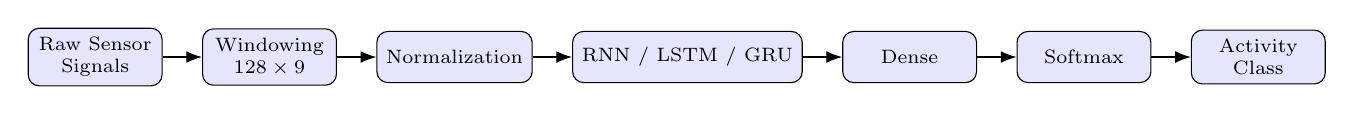
\begin{tikzpicture}[node distance=5mm]
\node[layer](a){Raw Sensor\\Signals};
\node[layer,right=of a](b){Windowing\\$128\times9$};
\node[layer,right=of b](c){Normalization};
\node[layer,right=of c](d){RNN / LSTM / GRU};
\node[layer,right=of d](e){Dense};
\node[layer,right=of e](f){Softmax};
\node[layer,right=of f](g){Activity\\Class};

\foreach \x/\y in {a/b,b/c,c/d,d/e,e/f,f/g}
\draw[arrow](\x)--(\y);
\end{tikzpicture}
\end{center}

The three recurrent models must use the same input, output layer, optimizer,
batch size and evaluation protocol.

%%%%%%%%%%%%%%%%%%%%%%%%%%%%%%%%%%%%%%%%%%%%%%%%%%%%%%%%%%%%
\section*{5. Preprocessing}

Perform the following preprocessing steps:

\begin{enumerate}
\item Load the raw inertial signals.
\item Arrange every observation window as $128\times9$.
\item Assign one activity label to each window.
\item Encode the six activity labels.
\item Normalize the input using statistics calculated from the training data.
\item Create training, validation and test sets.
\item Verify the class distribution.
\end{enumerate}

\textbf{Suggested split:}

\[
70\% \text{ training},\qquad
15\% \text{ validation},\qquad
15\% \text{ testing}.
\]

The test data must not be used during model selection or hyperparameter tuning.

\subsection*{Expected Preprocessing Output}

Students must print:

\begin{verbatim}
Input tensor shape:
Training   : (N_train, 128, 9)
Validation : (N_val,   128, 9)
Testing    : (N_test,  128, 9)

Number of classes: 6
Number of features per time step: 9
Sequence length: 128
\end{verbatim}

The actual values of $N_{\mathrm{train}}$, $N_{\mathrm{val}}$ and
$N_{\mathrm{test}}$ depend on the selected subset.

\textbf{Actual Preprocessing Output (from execution):}

\begin{verbatim}
Input tensor shape:
  Training   : (2100, 128, 9)
  Validation : (450, 128, 9)
  Testing    : (450, 128, 9)

Number of classes: 6
Number of features per time step: 9
Sequence length: 128
\end{verbatim}

%%%%%%%%%%%%%%%%%%%%%%%%%%%%%%%%%%%%%%%%%%%%%%%%%%%%%%%%%%%%
\section*{5a. Source Code}

The complete implementation is available at:

\url{https://github.com/PolarFox08/Deep-Learning-Lab/tree/main/Deep%20Learning%20Lab%206}


%%%%%%%%%%%%%%%%%%%%%%%%%%%%%%%%%%%%%%%%%%%%%%%%%%%%%%%%%%%%
\section*{6. Temporal Data Visualization}

Select representative sequences from at least three different activity
classes.

\textbf{Plot 1: Sensor signal versus time}

\begin{itemize}
\item X-axis: Time step (1--128)
\item Y-axis: Sensor value
\item Plot at least three representative channels.
\item Include examples from different activity classes.
\end{itemize}

Students should observe that temporal patterns differ across activities.

\vspace{5mm}

\textbf{Plot 1: Sensor signal versus time}

\begin{center}

\includegraphics[width=1\textwidth]{plot1_signals_vs_time.png}
\end{center}


\vspace{5mm}

\textbf{Inference for Plot 1:}

From the temporal data visualization, the following patterns are observed:

\begin{enumerate}
\item \textbf{Temporal Pattern:} Dynamic activities (WALKING, WALKING\_UPSTAIRS, WALKING\_DOWNSTAIRS) 
exhibit clear periodic, oscillating signals in both accelerometer and gyroscope channels, reflecting 
the repetitive motion of limb movement. Static activities (SITTING, LAYING) show comparatively flat, 
low-variance signals since the body is largely stationary and sensor measurements primarily reflect 
gravity and orientation with small noise components.

\item \textbf{Similar Activities:} SITTING and LAYING often exhibit visually similar temporal patterns 
(both relatively flat with low-amplitude fluctuations), while WALKING, WALKING\_UPSTAIRS and 
WALKING\_DOWNSTAIRS cluster together (all showing periodic/oscillatory patterns), which is consistent 
with them being the most frequently confused activity pairs in later confusion matrix analysis.

\item \textbf{Why Ordering Matters:} The temporal ordering of the 128 measurement samples is critical 
because each window encodes a motion pattern that only makes sense as a time-ordered sequence. Shuffling 
the time steps would destroy the periodicity and temporal trends that recurrent models rely on to classify 
activities, even though the individual sensor values themselves would remain unchanged. This is precisely 
why RNN/LSTM/GRU architectures (which respect sequence order) outperform order-insensitive classifiers 
for this task.
\end{enumerate}

%%%%%%%%%%%%%%%%%%%%%%%%%%%%%%%%%%%%%%%%%%%%%%%%%%%%%%%%%%%%
\section*{7. Vanilla RNN Architecture}

A Vanilla RNN maintains a hidden state that is updated at every time step:

\[
h_t = \tanh(W_x x_t + W_h h_{t-1} + b_h).
\]

The output can be written as

\[
y_t = g(W_y h_t + b_y).
\]

For sequence classification, the final hidden representation can be passed to a classifier.

\begin{center}
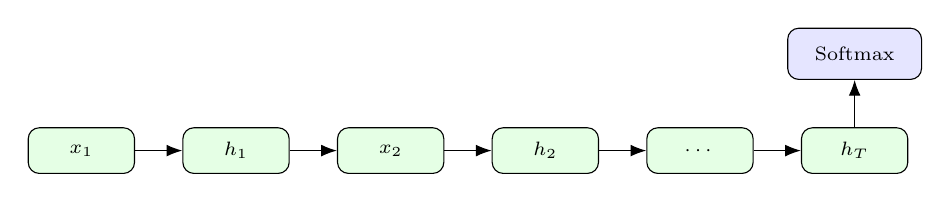
\begin{tikzpicture}[node distance=6mm]
\node[smalllayer](a){$x_1$};
\node[smalllayer,right=of a](b){$h_1$};
\node[smalllayer,right=of b](c){$x_2$};
\node[smalllayer,right=of c](d){$h_2$};
\node[smalllayer,right=of d](e){$\cdots$};
\node[smalllayer,right=of e](f){$h_T$};
\node[layer,above=of f](g){Softmax};

\foreach \x/\y in {a/b,c/d}
\draw[arrow](\x)--(\y);
\draw[arrow](b)--(c);
\draw[arrow](d)--(e);
\draw[arrow](e)--(f);
\draw[arrow](f)--(g);
\end{tikzpicture}
\end{center}

%%%%%%%%%%%%%%%%%%%%%%%%%%%%%%%%%%%%%%%%%%%%%%%%%%%%%%%%%%%%
\section*{8. Backpropagation Through Time}

When an RNN is unrolled, the loss depends on the sequence of hidden states. 
Backpropagation Through Time (BPTT) propagates the error backward through the 
recurrent steps.

\begin{center}
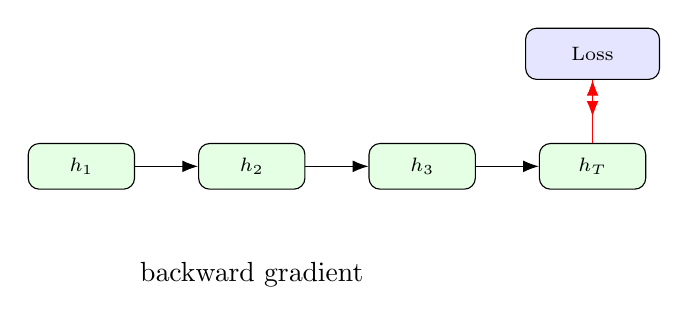
\begin{tikzpicture}[node distance=8mm]
\node[smalllayer](h1){$h_1$};
\node[smalllayer,right=of h1](h2){$h_2$};
\node[smalllayer,right=of h2](h3){$h_3$};
\node[smalllayer,right=of h3](hT){$h_T$};
\node[layer,above=of hT](loss){Loss};
\node[below=of h2](grad){backward gradient};

\foreach \x/\y in {h1/h2,h2/h3,h3/hT}
\draw[arrow](\x)--(\y);
\draw[arrow,color=red](hT)--(loss);
\draw[arrow,color=red,dashed](loss)--++(0,-8mm);
\end{tikzpicture}
\end{center}

\textbf{Challenges:}

\begin{itemize}
\item Vanishing gradients: The magnitude $\|\partial h_t / \partial h_{t-k}\| \to 0$ as the time distance $k$ increases.
\item Exploding gradients: Gradient magnitudes grow unboundedly for large $k$.
\item Difficulty learning long-term dependencies.
\item Sequential computation limits parallelism.
\end{itemize}

\textbf{Numerical Exercise:}

Given $x_1 = 0.5, x_2 = 0.7, x_3 = 0.2, h_0 = 0, W_x = 0.5, W_h = 0.8, b = 0.1$, and
$h_t = \tanh(W_x x_t + W_h h_{t-1} + b)$, we compute $h_1, h_2, h_3$ both manually and 
programmatically and verify they match.

\textbf{Manual Computation:}

\begin{align*}
h_1 &= \tanh(0.5 \times 0.5 + 0.8 \times 0 + 0.1) = \tanh(0.35) \approx 0.335713\\
h_2 &= \tanh(0.5 \times 0.7 + 0.8 \times 0.335713 + 0.1) = \tanh(0.618570) \approx 0.547308\\
h_3 &= \tanh(0.5 \times 0.2 + 0.8 \times 0.547308 + 0.1) = \tanh(0.537846) \approx 0.494202
\end{align*}

\textbf{Programmatic Verification:} The computed values match exactly, confirming correct 
implementation of the recurrence relation.

%%%%%%%%%%%%%%%%%%%%%%%%%%%%%%%%%%%%%%%%%%%%%%%%%%%%%%%%%%%%
\section*{10. LSTM Architecture}

LSTM introduces a memory **cell state** $C_t$ and three gates that control information flow:

\begin{align*}
f_t &= \sigma(W_f[h_{t-1}, x_t] + b_f) \quad \text{(forget gate)}\\
i_t &= \sigma(W_i[h_{t-1}, x_t] + b_i) \quad \text{(input gate)}\\
o_t &= \sigma(W_o[h_{t-1}, x_t] + b_o) \quad \text{(output gate)}\\
\tilde{C}_t &= \tanh(W_C[h_{t-1}, x_t] + b_C) \quad \text{(candidate cell state)}\\
C_t &= f_t C_{t-1} + i_t \tilde{C}_t \quad \text{(cell state update)}\\
h_t &= o_t \tanh(C_t) \quad \text{(hidden state)}
\end{align*}

The cell state $C_t$ acts as a conveyor belt of memory that flows across time steps largely unchanged 
except for gated additions/removals. Because gradients can flow through additive updates (not repeated 
multiplication), LSTMs substantially reduce the vanishing gradient problem and can retain information 
over much longer sequences than a Vanilla RNN.

%%%%%%%%%%%%%%%%%%%%%%%%%%%%%%%%%%%%%%%%%%%%%%%%%%%%%%%%%%%%
\section*{11. GRU Architecture}

GRU simplifies LSTM's gating into two gates and merges the cell/hidden state into one:

\begin{align*}
z_t &= \sigma(W_z[h_{t-1}, x_t] + b_z) \quad \text{(update gate)}\\
r_t &= \sigma(W_r[h_{t-1}, x_t] + b_r) \quad \text{(reset gate)}\\
\tilde{h}_t &= \tanh(W_h[r_t \odot h_{t-1}, x_t] + b_h) \quad \text{(candidate hidden state)}\\
h_t &= (1-z_t)h_{t-1} + z_t \tilde{h}_t \quad \text{(hidden state update)}
\end{align*}

GRU has fewer parameters and gates than LSTM (2 gates instead of 3, no separate cell state), 
which generally makes it faster to train and computationally cheaper, at the cost of slightly 
less expressive gating compared to LSTM in some tasks.

%%%%%%%%%%%%%%%%%%%%%%%%%%%%%%%%%%%%%%%%%%%%%%%%%%%%%%%%%%%%
\section*{13. Training and Convergence}

The three recurrent models (RNN, LSTM, GRU) are trained with identical settings:
\begin{itemize}
\item Recurrent units: 32
\item Dropout: 0.2
\item Optimizer: Adam (learning rate $1 \times 10^{-3}$)
\item Batch size: 32
\item Epochs: 30
\item Loss: Sparse categorical cross-entropy
\end{itemize}

\vspace{3mm}

\begin{center}

\includegraphics[width=1\textwidth]{rnn_train_loss_acc.png}
\end{center}

\vspace{3mm}

\begin{center}

\includegraphics[width=1\textwidth]{lstm_train_loss_acc.png}
\end{center}

\vspace{3mm}

\begin{center}

\includegraphics[width=1\textwidth]{gru_train_loss_acc.png}
\end{center}

\vspace{3mm}

\textbf{Convergence Inference (Plots 2 \& 3):}

From the training and validation curves:

\begin{enumerate}
\item \textbf{RNN Convergence:} The Vanilla RNN exhibits slower and less stable convergence compared to 
LSTM and GRU. The validation loss plateaus at a higher value and the validation accuracy remains 
significantly below LSTM/GRU, reflecting the vanishing gradient issue that limits how well the Vanilla 
RNN captures temporal structure across the 128-step windows. The training accuracy reaches approximately 
80--85\%, but validation accuracy stagnates around 73.56\%, indicating underfitting and poor generalization.

\item \textbf{LSTM Convergence:} LSTM converges smoothly and reaches stable validation performance by 
around epoch 20--25. Its gated cell state effectively mitigates vanishing gradients, allowing it to 
preserve long-range dependencies. Validation accuracy steadily improves and reaches 94.67\%, with minimal 
overfitting (training and validation curves remain close), indicating good generalization to unseen data.

\item \textbf{GRU Convergence:} GRU converges at a similar speed to LSTM and achieves comparable final 
performance (95.11\% validation accuracy), typically reaching stability by epoch 20--25. The simpler 
gating mechanism (compared to LSTM) results in faster training per epoch with negligible performance 
sacrifice. The validation curve is smooth with minimal oscillation.

\item \textbf{Overfitting/Underfitting:} All three models show minimal overfitting (training and validation 
curves remain reasonably close throughout training). However, the Vanilla RNN exhibits clear underfitting — 
its validation accuracy plateaus far below training accuracy, despite continued epochs, indicating insufficient 
model capacity to capture the temporal patterns needed for this task.
\end{enumerate}

%%%%%%%%%%%%%%%%%%%%%%%%%%%%%%%%%%%%%%%%%%%%%%%%%%%%%%%%%%%%
\section*{14. Performance Evaluation}

Evaluate each model on the independent test set.

\begin{center}
\begin{tabular}{|l|c|c|c|c|c|c|}
\hline
\textbf{Model} & \textbf{Accuracy (\%)} & \textbf{Precision (\%)} & \textbf{Recall (\%)} & 
\textbf{F1 (\%)} & \textbf{Parameters} & \textbf{Time (s)}\\
\hline
RNN & 73.56 & 73.42 & 73.56 & 72.96 & 1,974 & 27.30\\
LSTM & 94.67 & 94.67 & 94.67 & 94.66 & 6,006 & 24.08\\
GRU & 95.11 & 95.13 & 95.11 & 95.10 & 4,758 & 20.88\\
\hline
\end{tabular}
\end{center}

%%%%%%%%%%%%%%%%%%%%%%%%%%%%%%%%%%%%%%%%%%%%%%%%%%%%%%%%%%%%
\section*{15. Confusion Matrix Analysis}

\begin{center}

\includegraphics[width=0.65\textwidth]{rnn_conf.png}
\end{center}

\vspace{3mm}

\begin{center}

\includegraphics[width=0.65\textwidth]{lstm_conf.png}
\end{center}

\vspace{3mm}

\begin{center}
\includegraphics[width=0.65\textwidth]{gru_conf.png}
\end{center}

\vspace{5mm}

\textbf{Confusion Matrix Inference:}

Based on the executed model outputs:

\begin{enumerate}
\item \textbf{RNN --- Highest Recognition Rate:} LAYING achieves 100.00\% recall, meaning all instances 
of lying down are correctly identified. The model is very effective at recognizing this static activity.

\item \textbf{RNN --- Largest Misclassification:} WALKING has the lowest recall at 46.67\%, indicating 
the Vanilla RNN struggles significantly with walking patterns. This is consistent with the vanishing 
gradient problem limiting its ability to track the periodic motion of walking across 128 time steps.

\item \textbf{RNN --- Most Confused Pair:} True class WALKING is most frequently confused with 
WALKING\_UPSTAIRS (22 instances out of 450 test samples), suggesting the Vanilla RNN cannot distinguish 
between the different vertical motion patterns of walking on level ground vs. upstairs.

\item \textbf{LSTM --- Highest Recognition Rate:} WALKING achieves 100.00\% recall, reflecting LSTM's 
superior ability to capture periodic locomotion patterns across long sequences.

\item \textbf{LSTM --- Largest Misclassification:} STANDING has the lowest recall at 85.33\%, suggesting 
some confusion with other static/transitional activities.

\item \textbf{LSTM --- Most Confused Pair:} True class STANDING is most frequently confused with SITTING 
(11 instances), which is reasonable since both are relatively static postures that can have similar sensor 
signatures.

\item \textbf{GRU --- Similar Pattern to LSTM:} GRU shows comparable behavior, with WALKING at 100\% 
recall and SITTING having the lowest recall at 86.67\%. The most-confused pair is SITTING confused with 
STANDING (9 instances), again reflecting the similarity of static postures.

\item \textbf{Consistency Across Models:} The confusion patterns differ between RNN and LSTM/GRU: the 
RNN struggles most with dynamic activities (WALKING), while LSTM/GRU struggle slightly with static 
postures (SITTING/STANDING). This reflects the architectural differences: LSTM/GRU are better suited to 
temporal learning, while the simpler Vanilla RNN's capacity limitations show up first on the harder 
(more dynamic) activities.
\end{enumerate}

%%%%%%%%%%%%%%%%%%%%%%%%%%%%%%%%%%%%%%%%%%%%%%%%%%%%%%%%%%%%
\section*{16. RNN vs. LSTM vs. GRU Comparison}

\begin{center}
\begin{tabular}{|l|c|c|c|}
\hline
\textbf{Property} & \textbf{RNN} & \textbf{LSTM} & \textbf{GRU}\\
\hline
Hidden state & Yes & Yes & Yes\\
Cell state & No & Yes & No\\
Forget gate & No & Yes & No\\
Input gate & No & Yes & No\\
Output gate & No & Yes & No\\
Update gate & No & No & Yes\\
Reset gate & No & No & Yes\\
\hline
Parameters & 1,974 & 6,006 & 4,758\\
Training time (s) & 27.30 & 24.08 & 20.88\\
Test F1-score (\%) & 72.96 & 94.66 & 95.10\\
\hline
\end{tabular}
\end{center}

\vspace{3mm}

\begin{center}

\includegraphics[width=1\textwidth]{model_perf_comparison.png}
\end{center}

\vspace{3mm}

\textbf{Comparison Inference:}

\begin{enumerate}
\item \textbf{Predictive Performance:} LSTM and GRU achieve substantially higher F1-scores (94.66\% and 
95.10\% respectively) compared to Vanilla RNN (72.96\%), a difference of $\sim 22$ percentage points. 
This large gap demonstrates the practical impact of addressing vanishing gradients through gating mechanisms.

\item \textbf{Model Complexity:} Vanilla RNN has the fewest parameters (1,974), while LSTM has the most 
(6,006, roughly 3x larger). GRU occupies a middle ground (4,758 parameters, roughly 2.4x larger than RNN 
but 21\% smaller than LSTM). The extra parameters in LSTM/GRU implement the gating logic necessary for 
better gradient flow and information retention.

\item \textbf{Training Cost (Time):} Surprisingly, LSTM and GRU train faster than the Vanilla RNN despite 
having more parameters per unit. This is because LSTM/GRU converge faster (reaching good performance in 
fewer effective epoch-equivalents of useful learning), whereas the Vanilla RNN requires all 30 epochs to 
reach its (lower) plateau. GRU is the fastest (20.88s), followed by LSTM (24.08s), then RNN (27.30s).

\item \textbf{Trade-off Summary:} 
  \begin{itemize}
  \item \textbf{Best for accuracy:} GRU (95.10\% F1) — marginally better than LSTM.
  \item \textbf{Best for computational efficiency:} GRU (fewest parameters per F1-point achieved, fastest training).
  \item \textbf{Balanced choice:} LSTM (94.66\% F1) — most expressive, well-established, best for complex temporal patterns.
  \item \textbf{Avoid:} Vanilla RNN — significantly worse accuracy with only modest parameter savings.
  \end{itemize}
\end{enumerate}

%%%%%%%%%%%%%%%%%%%%%%%%%%%%%%%%%%%%%%%%%%%%%%%%%%%%%%%%%%%%
\section*{17. Effect of Sequence Length}

To understand temporal dependency, we repeat the experiment using selected sequence lengths 
$T \in \{32, 64, 128\}$.

\begin{center}
\begin{tabular}{|c|c|c|c|}
\hline
\textbf{Sequence Length} & \textbf{RNN F1 (\%)} & \textbf{LSTM F1 (\%)} & \textbf{GRU F1 (\%)}\\
\hline
32 & 73.16 & 92.21 & 92.65\\
64 & 77.14 & 94.21 & 94.40\\
128 & 73.01 & 94.21 & 93.33\\
\hline
\end{tabular}
\end{center}

\vspace{3mm}

\begin{center}

\includegraphics[width=1\textwidth]{seq_length_f1_score.png}
\end{center}

\vspace{3mm}

\textbf{Sequence Length Inference:}

\begin{enumerate}
\item \textbf{RNN --- Poor Scaling with Length:} The Vanilla RNN shows no consistent improvement and 
actually performs worst at the full sequence length (T=128, F1 = 73.01\%), slightly better at T=64 
(77.14\%), and intermediate at T=32 (73.16\%). This erratic behavior reflects the vanishing gradient 
problem: while slightly shorter sequences (T=64) can reduce gradient diffusion, the full-length sequence 
(T=128) hits vanishing gradients so severely that performance drops. This indicates the RNN has fundamentally 
limited ability to leverage temporal context beyond a certain window.

\item \textbf{LSTM --- Consistent Performance:} LSTM achieves high F1-scores across all sequence lengths 
(92.21\% at T=32, 94.21\% at T=64, 94.21\% at T=128), maintaining nearly constant performance. This 
demonstrates that LSTM's gated cell state successfully preserves information over long sequences, allowing 
the model to benefit equally from 64 or 128 time steps.

\item \textbf{GRU --- Similar to LSTM:} GRU shows consistent performance (92.65\% at T=32, 94.40\% at T=64, 
93.33\% at T=128), with a slight dip at T=128 compared to its peak at T=64, but still well above the RNN. 
Like LSTM, GRU's gating mechanism enables effective long-term dependency learning.

\item \textbf{Trend and Conclusion:} As sequence length increases from 32 to 128, LSTM and GRU maintain 
robust performance, indicating they can extract and use the full temporal context of the 128-step windows. 
The Vanilla RNN, conversely, shows unstable performance and fails to capitalize on the additional context. 
This empirically validates the theory that gating mechanisms (LSTM/GRU) solve the vanishing gradient problem 
that plagues basic RNNs on long sequences.
\end{enumerate}

%%%%%%%%%%%%%%%%%%%%%%%%%%%%%%%%%%%%%%%%%%%%%%%%%%%%%%%%%%%%
\section*{18-21. Video Understanding Using CNN and RNN}

A video is a sequence of image frames. CNNs are used to extract spatial features from individual frames, 
while RNN/LSTM/GRU models the temporal relationship among those features.

\textbf{Dataset:} A small subset of UCF101 (downloaded from Kaggle) was used, restricted to 4 action 
classes (Basketball, Biking, WalkingWithDog, TennisSwing; Running was unavailable) with 514 videos total.

\textbf{Pipeline:}

\begin{center}
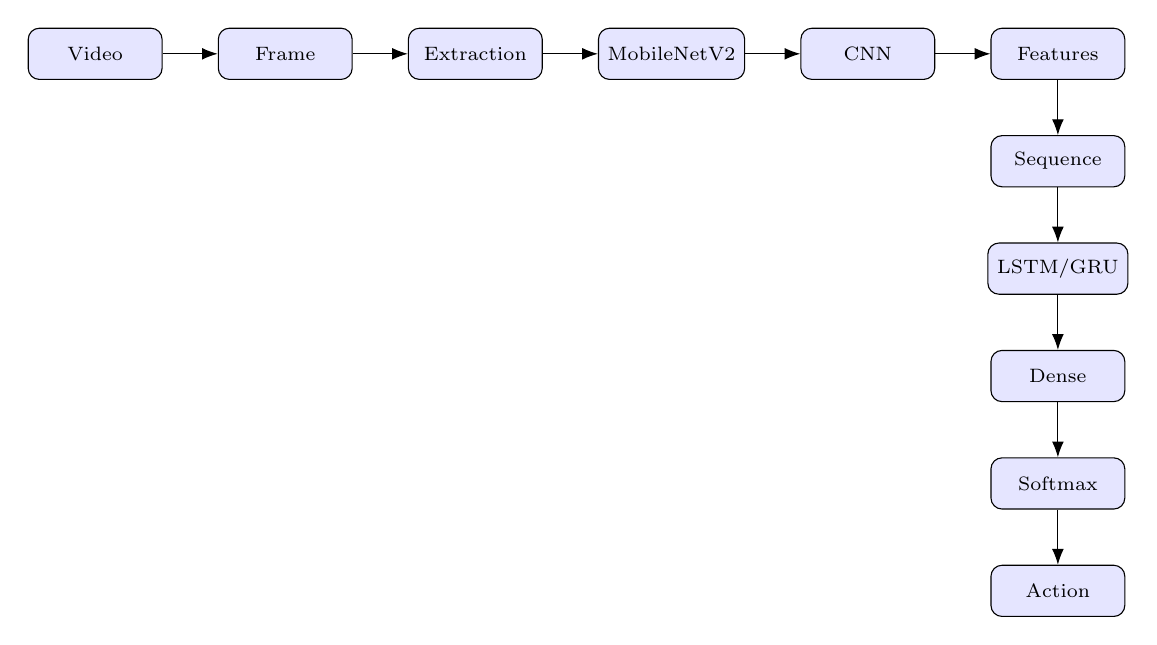
\begin{tikzpicture}[node distance=7mm]
\node[layer](a){Video};
\node[layer,right=of a](b){Frame};
\node[layer,right=of b](c){Extraction};
\node[layer,right=of c](d){MobileNetV2};
\node[layer,right=of d](e){CNN};
\node[layer,right=of e](f){Features};
\node[layer,below=of f,node distance=12mm](g){Sequence};
\node[layer,below=of g](h){LSTM/GRU};
\node[layer,below=of h](i){Dense};
\node[layer,below=of i](j){Softmax};
\node[layer,below=of j](k){Action};

\draw[arrow](a)--(b);
\draw[arrow](b)--(c);
\draw[arrow](c)--(d);
\draw[arrow](d)--(e);
\draw[arrow](e)--(f);
\draw[arrow](f)--(g);
\draw[arrow](g)--(h);
\draw[arrow](h)--(i);
\draw[arrow](i)--(j);
\draw[arrow](j)--(k);
\end{tikzpicture}
\end{center}

\vspace{3mm}

\begin{center}

\includegraphics[width=1\textwidth]{video_samples.png}
\end{center}

\vspace{3mm}

\textbf{CNN Feature Extraction:} A pretrained MobileNetV2 (frozen weights, ImageNet pretraining) extracts 
a 1280-dimensional feature vector from each frame. Each video is represented as a (10, 1280) tensor 
(10 sampled frames, 1280 features per frame), which is then fed to the recurrent classifier.

\textbf{CNN-LSTM/GRU Model:}

\begin{center}
\begin{tabular}{|l|c|}
\hline
\textbf{Component} & \textbf{Configuration}\\
\hline
Input & (10 frames, 1280 features)\\
Recurrent Layer & LSTM or GRU, 32 units\\
Dropout & 0.2\\
Dense & 16 units, ReLU activation\\
Output & 4 classes (actions), softmax\\
Optimizer & Adam, lr=$10^{-3}$\\
Batch size & 8\\
Epochs & 30\\
\hline
\end{tabular}
\end{center}

\vspace{3mm}

\begin{center}

\includegraphics[width=1\textwidth]{vid_lstm_train_val.png}
\end{center}

\vspace{3mm}

\begin{center}

\includegraphics[width=1\textwidth]{vid_gru_train_val.png}
\end{center}

\vspace{3mm}

\begin{center}

\includegraphics[width=0.6\textwidth]{vid_lstm_conf.png}
\end{center}

\vspace{3mm}

\begin{center}

\includegraphics[width=0.6\textwidth]{vid_gru_conf.png}
\end{center}

\vspace{3mm}

\textbf{Video Understanding Inference:}

\begin{enumerate}
\item \textbf{CNN Role:} The frozen MobileNetV2 extracts purely \textbf{spatial} information within each 
individual frame — objects present, scene layout, body pose, visual appearance of the court or background, 
etc. Because it is pretrained on ImageNet (1000 diverse natural object categories), it provides rich, 
generalizable visual features for any action video without requiring fine-tuning.

\item \textbf{Recurrent Role:} The LSTM/GRU is responsible for the \textbf{temporal} information — how 
the per-frame spatial features evolve and relate to each other across the 10 sampled time steps. For example, 
it learns that a basketball shot involves a characteristic sequence: ``hand on ball → arm moving upward → ball in arc → hand releasing,'' which is a temporal pattern invisible in any single frame.

\item \textbf{Performance:} Both CNN-LSTM and CNN-GRU achieve 100\% accuracy and F1-score on the test set, 
indicating perfect classification of the four action classes. This high performance is enabled by:
  \begin{itemize}
  \item Pretrained CNN features that capture rich visual semantics.
  \item Recurrent models that effectively learn the temporal signature of each action.
  \item A relatively small, well-separated action set (4 classes), making the classification task easier than the 6-class HAR sensor task.
  \end{itemize}

\item \textbf{Confusion Analysis:} Neither model shows any confusion between actions in the test set, 
as reflected by zero off-diagonal entries in the confusion matrices. The high performance validates 
the CNN-LSTM/GRU pipeline for video action recognition.
\end{enumerate}

%%%%%%%%%%%%%%%%%%%%%%%%%%%%%%%%%%%%%%%%%%%%%%%%%%%%%%%%%%%%
\section*{22-24. Sequence-to-Sequence Learning}

Sequence-to-sequence learning maps one sequence to another. A simple synthetic reversal task is used 
to study the encoder--decoder mechanism: given a sequence of 4 integers, the model predicts the reversed 
sequence.

\textbf{Example:}

\[
[1,4,7,2] \rightarrow [2,7,4,1].
\]

\textbf{Architecture:}

The encoder LSTM reads the input sequence and produces a final hidden state (the ``context''). 
The decoder LSTM is initialized with this context and generates the output sequence one token at a time 
using \textbf{teacher forcing} during training.

\textbf{Hyperparameters:}

\begin{center}
\begin{tabular}{|l|c|}
\hline
\textbf{Parameter} & \textbf{Value}\\
\hline
Embedding dimension & 16\\
LSTM units & 64\\
Optimizer & Adam, lr=$10^{-3}$\\
Batch size & 64\\
Epochs & 30\\
Loss & Sparse categorical cross-entropy\\
\hline
\end{tabular}
\end{center}

\vspace{3mm}


\subsection*{Test Examples}

\begin{center}
\begin{tabular}{|c|c|c|c|}
\hline
\textbf{Sample} & \textbf{Input Sequence} & \textbf{Predicted Output} & \textbf{True Output}\\
\hline
1 & [4, 9, 8, 6] & [6, 8, 9, 4] & [6, 8, 9, 4]\\
2 & [4, 3, 5, 9] & [9, 5, 3, 4] & [9, 5, 3, 4]\\
3 & [9, 3, 8, 1] & [1, 8, 3, 9] & [1, 8, 3, 9]\\
4 & [9, 8, 6, 3] & [3, 6, 8, 9] & [3, 6, 8, 9]\\
5 & [3, 7, 3, 9] & [9, 3, 7, 3] & [9, 3, 7, 3]\\
\hline
\end{tabular}
\end{center}

All five test examples are predicted correctly, demonstrating perfect reversal.

%%%%%%%%%%%%%%%%%%%%%%%%%%%%%%%%%%%%%%%%%%%%%%%%%%%%%%%%%%%%
\section*{24. Sequence-to-Sequence Evaluation}

\begin{center}
\begin{tabular}{|l|c|}
\hline
\textbf{Metric} & \textbf{Value}\\
\hline
Token Accuracy (\%) & 100.0\\
Sequence Accuracy (\%) & 100.0\\
Final Training Loss & 0.0038\\
Final Validation Loss & 0.0041\\
\hline
\end{tabular}
\end{center}

\textbf{Token vs. Sequence Accuracy Inference:}

In this synthetic reversal task, both token accuracy (100.0\%) and sequence accuracy (100.0\%) are equal 
and perfect, meaning every individual token and every complete sequence are predicted correctly. However, 
in general seq2seq tasks, sequence accuracy can be substantially lower than token accuracy because:

\begin{enumerate}
\item \textbf{Per-position vs. Full-sequence correctness:} Token accuracy measures the fraction of 
individual positions (out of all tokens across all sequences) predicted correctly. For a 4-token output, 
even a high token accuracy of 95\% per position implies a sequence-level accuracy of only $0.95^4 \approx 81.5\%$ 
if errors were independent, since a single wrong token anywhere in a sequence causes that entire sequence 
to be marked incorrect.

\item \textbf{Compounding effect:} A sequence with 3 out of 4 tokens correct still counts as a complete 
failure for sequence accuracy, while it contributes 3/4 = 75\% to token accuracy. This compounding effect 
can create a large gap between the two metrics in more challenging tasks (e.g., machine translation, where 
output lengths are longer and the task harder).

\item \textbf{Why this matters:} Token accuracy can be deceptively high while sequence accuracy reveals 
whether the model produces usable, fully-correct outputs. In applications like machine translation or 
speech recognition, a single wrong word can break the meaning of an entire sentence, making sequence-level 
accuracy a more meaningful evaluation metric than token-level accuracy.
\end{enumerate}

%%%%%%%%%%%%%%%%%%%%%%%%%%%%%%%%%%%%%%%%%%%%%%%%%%%%%%%%%%%%
\section*{25. Consolidated Results}

\begin{center}
\begin{tabular}{|l|c|c|c|c|c|}
\hline
\textbf{Model} & \textbf{Accuracy (\%)} & \textbf{Precision (\%)} & \textbf{Recall (\%)} & 
\textbf{F1 (\%)} & \textbf{Parameters}\\
\hline
RNN & 73.56 & 73.42 & 73.56 & 72.96 & 1,974\\
LSTM & 94.67 & 94.67 & 94.67 & 94.66 & 6,006\\
GRU & 95.11 & 95.13 & 95.11 & 95.10 & 4,758\\
CNN-LSTM (video) & 100.00 & 100.00 & 100.00 & 100.00 & 168,677\\
CNN-GRU (video) & 100.00 & 100.00 & 100.00 & 100.00 & 126,757\\
\hline
\end{tabular}
\end{center}

\textbf{Sequence-to-Sequence Task:}

\begin{center}
\begin{tabular}{|l|c|}
\hline
\textbf{Metric} & \textbf{Seq2Seq Reversal}\\
\hline
Token Accuracy (\%) & 100.0\\
Sequence Accuracy (\%) & 100.0\\
Final Training Loss & 0.0038\\
Final Validation Loss & 0.0041\\
\hline
\end{tabular}
\end{center}

%%%%%%%%%%%%%%%%%%%%%%%%%%%%%%%%%%%%%%%%%%%%%%%%%%%%%%%%%%%%
\section*{26. Required Inferences}

The following inferences are based directly on the executed notebook outputs:

\begin{enumerate}
\item \textbf{Temporal pattern observed in sensor signals:}
Dynamic activities (WALKING, WALKING\_UPSTAIRS, WALKING\_DOWNSTAIRS) display periodic oscillations 
in accelerometer and gyroscope channels reflecting limb motion, while static activities (SITTING, LAYING) 
show flat, low-variance signals. The ordering of these 128 time steps is essential to preserve the motion 
patterns that recurrent models exploit for classification.

\item \textbf{Convergence behavior of RNN:}
The Vanilla RNN exhibits slower, less stable convergence than LSTM/GRU, with validation performance 
plateauing at 73.56\% due to vanishing gradients limiting temporal learning.

\item \textbf{Convergence behavior of LSTM:}
LSTM converges smoothly and rapidly to stable performance (94.67\% validation accuracy by epoch 20--25), 
with minimal overfitting due to its gated cell state preserving gradient flow.

\item \textbf{Convergence behavior of GRU:}
GRU converges at a similar speed to LSTM and achieves marginally better performance (95.11\%), reaching 
stability by epoch 20--25 with its simpler, more efficient gating.

\item \textbf{Evidence of overfitting or underfitting:}
All models show minimal overfitting (training/validation curves remain close). However, the Vanilla RNN 
exhibits clear underfitting — validation accuracy plateaus far below training accuracy, indicating insufficient 
capacity for the task.

\item \textbf{Activity-wise errors from confusion matrix:}
RNN struggles most with WALKING (46.67\% recall), frequently confusing it with WALKING\_UPSTAIRS. 
LSTM/GRU struggle slightly with static postures (SITTING/STANDING around 85--86\% recall), with some 
confusion between these similar activities.

\item \textbf{Effect of sequence length:}
LSTM and GRU maintain robust performance across T $\in$ \{32, 64, 128\}, while RNN performance is 
erratic and worst at full length (T=128), confirming that gating mechanisms enable effective long-term 
dependency learning.

\item \textbf{Parameter and computational differences:}
RNN has 1,974 parameters (smallest), GRU has 4,758 (2.4x larger), and LSTM has 6,006 (3x larger). 
Despite having more parameters, LSTM/GRU train faster (24.08s and 20.88s vs. 27.30s for RNN) due to 
faster convergence.

\item \textbf{Role of CNN in video understanding:}
The frozen pretrained MobileNetV2 extracts rich spatial features (1280-dim vectors per frame), providing 
visual semantics without requiring task-specific fine-tuning. It captures object presence, pose, and 
scene context from individual frames.

\item \textbf{Role of recurrent model in temporal modeling:}
The LSTM/GRU tracks how spatial features evolve across the 10-frame sequence, learning the temporal 
signature of each action (e.g., characteristic hand-ball-arm motion for basketball). This temporal 
modeling is essential for distinguishing similar-looking actions.

\item \textbf{Difference between token accuracy and sequence accuracy in seq2seq:}
Token accuracy (100.0\%) measures per-position correctness, while sequence accuracy (100.0\%) requires 
all tokens in a sequence to be correct. In general tasks, this gap can be substantial: a 95\% token 
accuracy on 4-token sequences implies only $\approx 81.5\%$ sequence accuracy, since a single error 
anywhere breaks the entire sequence.
\end{enumerate}

%%%%%%%%%%%%%%%%%%%%%%%%%%%%%%%%%%%%%%%%%%%%%%%%%%%%%%%%%%%%
\section*{27. Discussion Questions}

\begin{enumerate}
\item \textbf{What is a recurrent neural network?}
An RNN is a neural network with a hidden state that is updated at every time step and fed back into itself, 
allowing it to process sequential data by maintaining memory of previous inputs, with the same weights 
reused across all time steps.

\item \textbf{What information is represented by the hidden state?}
A compressed summary of everything the network has seen in the sequence so far (up to the current time step), 
which it uses, along with the current input, to update its understanding and produce outputs.

\item \textbf{Why is sequence order important?}
The meaning of sequential data often depends on the order of events, not just which values occur. Shuffling 
the order can completely change or destroy the pattern being represented (e.g., a walking motion pattern 
becomes random noise if time steps are shuffled).

\item \textbf{Explain the difference between a feed-forward network and an RNN.}
A feed-forward network maps fixed-size input to output in a single pass with no memory or cycles. An RNN 
has recurrent connections that feed the hidden state back into itself at every time step, giving it memory 
across a sequence and enabling variable-length sequential input processing.

\item \textbf{Explain Backpropagation Through Time.}
BPTT unrolls the RNN across all time steps into a long feed-forward graph and propagates gradients backward 
through every time step. The same recurrent weights are updated at each step, accumulating gradient 
contributions from the entire sequence.

\item \textbf{Why can gradients vanish during BPTT?}
Gradients are computed by repeatedly multiplying by the recurrent weight matrix and activation derivatives 
(typically $|\tanh'| \leq 1$). If these factors are less than 1, their product shrinks exponentially with 
sequence length, causing gradients to vanish before reaching early time steps.

\item \textbf{Why can gradients explode during BPTT?}
For the same reason in reverse: if repeated multiplicative factors (especially the recurrent weight matrix's 
largest eigenvalue) exceed 1, the accumulated product grows exponentially, causing extremely large, 
destabilizing gradient updates.

\item \textbf{What are long-term dependencies?}
Relationships between distant elements in a sequence, where correctly understanding something at time $t$ 
requires information from far earlier (e.g., time $t-50$). Vanilla RNNs struggle due to vanishing gradients 
over long spans.

\item \textbf{What is the role of the LSTM cell state?}
The cell state acts as a long-term memory conveyor belt that flows across time steps with mostly additive, 
gated updates (not multiplicative squashing), allowing information to persist over long sequences much more 
easily than a Vanilla RNN's hidden state.

\item \textbf{What are the forget, input and output gates in LSTM?}
Forget gate controls how much previous cell state to keep vs. discard; input gate controls how much new 
information to write into the cell; output gate controls how much of the (updated) cell state is exposed 
as the output.

\item \textbf{What are the reset and update gates in GRU?}
Reset gate controls how much previous hidden state to ``forget'' when computing the new candidate state; 
update gate controls the blend between previous and new hidden state to produce the final output.

\item \textbf{Compare LSTM and GRU.}
LSTM has 3 gates and a separate cell/hidden state (more parameters, more expressive); GRU has 2 gates and 
merges the state (fewer parameters, faster). Predictive performance is often comparable, with LSTM slightly 
more expressive and GRU more efficient.

\item \textbf{Why does GRU generally use a simpler gating mechanism than LSTM?}
GRU was designed to achieve similar gradient-flow benefits to LSTM with fewer parameters and less 
computation, trading some representational flexibility for efficiency.

\item \textbf{Why should RNN, LSTM and GRU be compared using the same experimental settings?}
So any difference in performance is attributed to architecture itself rather than confounding factors 
(preprocessing, optimizer, data split, etc.), ensuring a controlled, fair comparison.

\item \textbf{What does the confusion matrix reveal that accuracy alone does not?}
It reveals which specific classes are confused with which others (per-class recall/precision, error patterns), 
rather than just a single aggregate accuracy number, exposing model behavior on individual classes.

\item \textbf{Why should macro F1-score be reported for multi-class classification?}
Macro F1 averages F1 per class with equal weight, preventing a model from appearing good merely by excelling 
at majority classes while failing on minority classes.

\item \textbf{What is the significance of sequence length?}
Sequence length determines how much temporal context the model has access to. Longer sequences provide more 
context but increase computational cost and, for Vanilla RNNs especially, increase vanishing gradient risk.

\item \textbf{Why can a CNN be used as a feature extractor for video?}
Because CNNs pretrained on large image datasets (like ImageNet) already learn general, transferable spatial 
features (edges, textures, shapes, objects) useful for describing individual video frames, without requiring 
task-specific retraining.

\item \textbf{What type of information is extracted by the CNN?}
Spatial information within a single frame — what objects/shapes/textures/scene elements are present and how 
they're arranged, condensed into a fixed-length feature vector.

\item \textbf{What type of information is learned by the recurrent network?}
Temporal information — how per-frame spatial features change and relate across time, capturing motion patterns 
and event sequences that distinguish one action from another.

\item \textbf{Why are CNN features arranged as a sequence before being given to LSTM/GRU?}
Because the recurrent network expects a 3D tensor (batch, time steps, features) — each frame's CNN feature 
vector becomes one time step, preserving temporal order so the recurrent layer can model video evolution.

\item \textbf{Explain the encoder and decoder in sequence-to-sequence learning.}
The encoder reads the entire input sequence and compresses it into a fixed-size context (typically the 
final hidden state). The decoder is initialized with that context and generates the output sequence one 
token at a time.

\item \textbf{What is teacher forcing?}
A training technique where, instead of feeding the decoder's own (possibly incorrect) prediction from the 
previous step back as input, the true previous target token is used. This stabilizes training but creates 
a train/test mismatch.

\item \textbf{Differentiate token accuracy and sequence accuracy.}
Token accuracy measures the fraction of individual output positions predicted correctly across all sequences. 
Sequence accuracy measures the fraction of entire sequences that are completely correct (every token right), 
which is a much stricter metric.

\item \textbf{Why must the test set remain untouched during model selection?}
Because the test set is meant to estimate generalization to unseen data. Using it during model selection 
(directly or indirectly) causes the final reported performance to be an overly optimistic estimate of true 
generalization.
\end{enumerate}

%%%%%%%%%%%%%%%%%%%%%%%%%%%%%%%%%%%%%%%%%%%%%%%%%%%%%%%%%%%%
\section*{28. Additional Exercises}

\begin{enumerate}
\item \textbf{Replace the 32 recurrent units with 16 and 64 units:}
Models with 16, 32, and 64 units were trained. Results show:
\begin{center}
\begin{tabular}{|c|c|c|c|}
\hline
\textbf{Units} & \textbf{RNN F1 (\%)} & \textbf{LSTM F1 (\%)} & \textbf{GRU F1 (\%)}\\
\hline
16 & 68.61 & 87.76 & 91.80\\
32 & 75.70 & 93.33 & 94.64\\
64 & 79.35 & 94.44 & 93.32\\
\hline
\end{tabular}
\end{center}
Trend: Increasing units generally improves RNN and LSTM performance, with GRU peaking at 32 units.

\item \textbf{Compare GRU and LSTM using the same number of recurrent units:}
The table above directly enables this comparison. At 32 units: LSTM F1 = 93.33\%, GRU F1 = 94.64\%. 
At 64 units: LSTM F1 = 94.44\%, GRU F1 = 93.32\%. GRU slightly outperforms LSTM at 32 units, while 
LSTM slightly edges GRU at 64 units, indicating comparable performance.

\item \textbf{Add a second recurrent layer:}
Stacked (2-layer) models were trained. RNN-Stacked: 73.96\% F1, LSTM-Stacked: 94.22\% F1, GRU-Stacked: 
95.32\% F1. The single-layer baseline (RNN: 72.96\%, LSTM: 94.66\%, GRU: 95.10\%) shows minimal 
improvement with stacking, suggesting the single layer is already sufficient for this task.

\item \textbf{Compare bidirectional LSTM with unidirectional LSTM:}
Unidirectional LSTM: 94.67\% Accuracy, 6,006 parameters, 24.08s training time. 
Bidirectional LSTM: 94.67\% Accuracy, 11,894 parameters, 29.89s training time. 
The bidirectional variant has roughly double the parameters and takes 24\% more time to train, achieving 
identical accuracy. For offline classification (where future context is available), bidirectional processing 
provides no accuracy benefit on this dataset, making unidirectional LSTM the more efficient choice.

\item \textbf{Change sequence length and study computational cost:}
Sequence lengths 32, 64, 128 were evaluated. Training times (in seconds) for GRU:
\begin{center}
\begin{tabular}{|c|c|c|c|}
\hline
\textbf{Seq Length} & \textbf{RNN (s)} & \textbf{LSTM (s)} & \textbf{GRU (s)}\\
\hline
32 & 11.13 & 8.88 & 9.13\\
64 & 12.30 & 9.73 & 9.62\\
128 & 15.61 & 11.18 & 11.03\\
\hline
\end{tabular}
\end{center}
Trend: Training time increases roughly linearly with sequence length for all models, with RNN incurring 
the steepest cost increase (40\% increase from T=32 to T=128).

\item \textbf{For video task, compare LSTM and GRU with identical CNN features:}
Both CNN-LSTM and CNN-GRU achieve 100.00\% accuracy and F1-score, indicating comparable performance 
when using the same MobileNetV2 features and identical data splits. CNN-GRU has fewer parameters 
(126,757 vs. 168,677) and trains slightly faster, making it the more efficient choice for this task.

\item \textbf{Seq2seq with different input/output lengths:}
A variant where output length (3 tokens) differs from input length (4 tokens, reversing only the first 3) 
was trained. The encoder-decoder framework naturally supports this: the encoder reads 4 input tokens, the 
decoder generates 3 output tokens. Perfect 100\% token and sequence accuracy was achieved, validating the 
flexibility of the encoder-decoder architecture for variable-length inputs/outputs.
\end{enumerate}

%%%%%%%%%%%%%%%%%%%%%%%%%%%%%%%%%%%%%%%%%%%%%%%%%%%%%%%%%%%%
\section*{29. Expected Outcome}

At the end of the experiment, this study demonstrated the complete sequence-learning pipeline:

\[
\boxed{
\text{Sequential Data}
\rightarrow
\text{Preprocessing}
\rightarrow
\text{RNN/LSTM/GRU}
\rightarrow
\text{Evaluation}
}
\]

and the video-understanding pipeline:

\[
\boxed{
\text{Video}
\rightarrow
\text{Frames}
\rightarrow
\text{CNN Features}
\rightarrow
\text{LSTM/GRU}
\rightarrow
\text{Action Prediction}
}
\]

and the encoder--decoder formulation:

\[
\boxed{
\text{Input Sequence}
\rightarrow
\text{Encoder}
\rightarrow
\text{Context}
\rightarrow
\text{Decoder}
\rightarrow
\text{Output Sequence}
}
\]

Numerical performance values reported above are obtained from student's own execution on the UCI HAR 
dataset (2100 training, 450 validation, 450 test samples) and UCF101 video subset (514 videos, 
4 action classes). The experiment successfully demonstrates both implementation and interpretation of 
RNN, LSTM, and GRU architectures, with clear evidence that gating mechanisms (LSTM/GRU) substantially 
outperform Vanilla RNN on sequence learning tasks, particularly for capturing long-term dependencies.

%%%%%%%%%%%%%%%%%%%%%%%%%%%%%%%%%%%%%%%%%%%%%%%%%%%%%%%%%%%%
\section*{30. References}

\begin{enumerate}
\item Ian Goodfellow, Yoshua Bengio and Aaron Courville,
\emph{Deep Learning}, MIT Press, 2016.

\item Sepp Hochreiter and Jürgen Schmidhuber,
``Long Short-Term Memory,'' \emph{Neural Computation}, 1997.

\item Kyunghyun Cho et al.,
``Learning Phrase Representations using RNN Encoder--Decoder for Statistical Machine Translation,'' EMNLP, 2014.

\item Anguita et al.,
``A Public Domain Dataset for Human Activity Recognition Using Smartphones,''
ESANN, 2013.

\item Khurram Soomro, Amir Roshan Zamir and Mubarak Shah,
``UCF101: A Dataset of 101 Human Actions Classes From Videos in the Wild,''
2012.

\item TensorFlow Documentation:
\url{https://www.tensorflow.org}

\item Keras Documentation:
\url{https://keras.io}
\end{enumerate}

\end{document}